\documentclass{standalone}
\usepackage{tikz}
\usetikzlibrary{shapes,arrows,positioning}
\begin{document}
  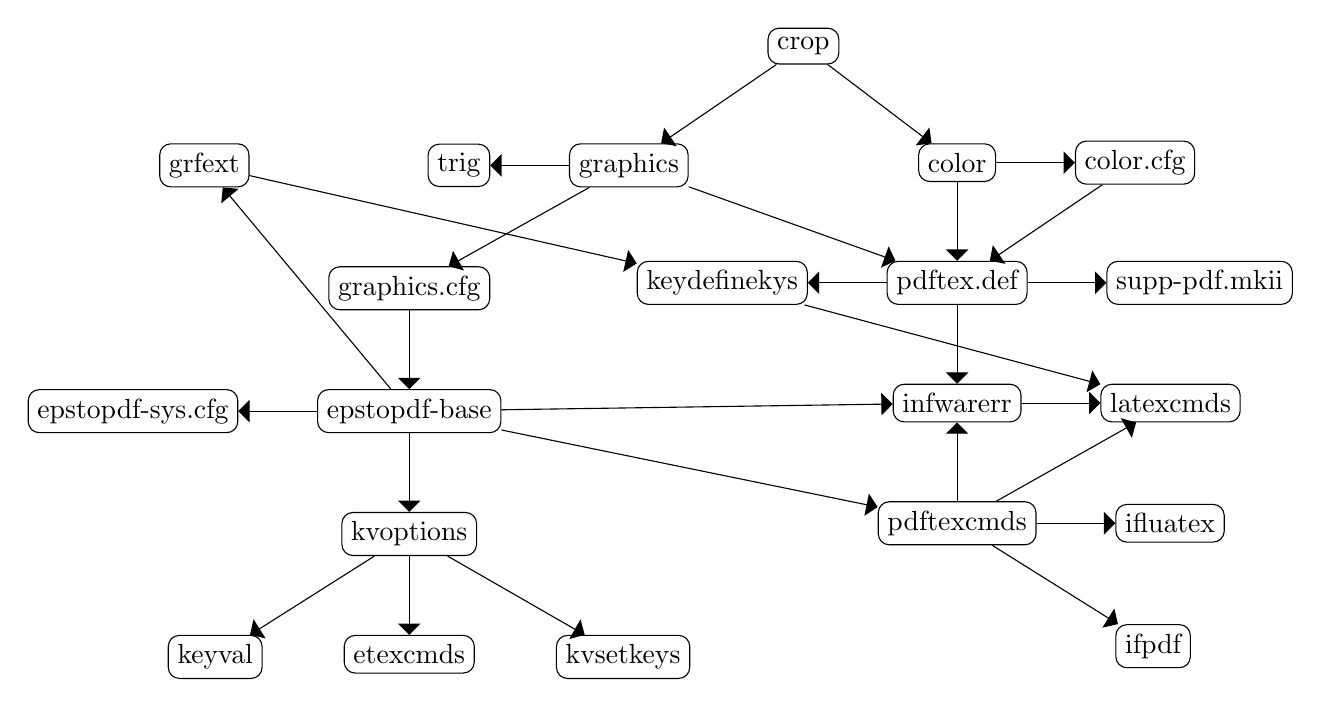
\begin{tikzpicture}
  
  \tikzset{main node/.style={rectangle, draw,
  		text centered, rounded corners}, }
  \tikzset{main verb/.style={minimum size=1cm}, }
  \tikzset{linea/.style={-triangle 90}, }
\node[main node] (1)   {crop};
\node[main node] (2) [below right =of 1]  {color};
\node[main node] (3) [right =of 2]  {color.cfg};
\node[main node] (4) [below =of 2]  {pdftex.def};
\node[main node] (11) [right =of 4]  {supp-pdf.mkii};
\node[main node] (5) [below=of 4]  {infwarerr};
\node[main node] (6) [ right =of 5]  {latexcmds};
\node[main node] (7) [below left =of 1]  {graphics};
\node[main node] (8) [left =of 7]  {trig};
\node[main node] (9) [below left =of 7]  {graphics.cfg};
\node[main node] (15) [below  =of 9]  {epstopdf-base};

\node[main node] (18) [below  =of 15]  {kvoptions};
\node[main node] (16) [above left  =of 9]  {grfext};
\node[main node] (17) [ left  =of 4]  {keydefinekys};
\node[main node] (12) [below   =of 5]  {pdftexcmds};
\node[main node] (13) [ right  =of 12]  {ifluatex};
\node[main node] (14) [below  right =of 12]  {ifpdf};
\node[main node] (19) [below left  =of 18]  {keyval};
\node[main node] (20) [below right  =of 18]  {kvsetkeys};
\node[main node] (21) [below   =of 18]  {etexcmds};
\node[main node] (22) [left   =of 15]  {epstopdf-sys.cfg};
\foreach \x /\y in{1/2,1/7,2/3,3/4,2/4,4/11,4/5,5/6,7/4,7/8,7/9,9/15,4/17,15/5,15/18,15/16,15/12,12/5,12/6,12/14,12/13,16/17,17/6,18/19,18/20,18/21,15/22}
  \path[linea] (\x) edge node {} (\y);
%%  
\end{tikzpicture}
\end{document}